%%%%%%%%%%%%%%%%%%%%%%%%%%%%%%%%%%%%%%%%%
% Cleese Assignment (For Students)
% LaTeX Template
% Version 2.0 (27/5/2018)
%
% This template originates from:
% http://www.LaTeXTemplates.com
%
% Author:
% Vel (vel@LaTeXTemplates.com)
%
% License:
% CC BY-NC-SA 3.0 (http://creativecommons.org/licenses/by-nc-sa/3.0/)
% 
%%%%%%%%%%%%%%%%%%%%%%%%%%%%%%%%%%%%%%%%%

%----------------------------------------------------------------------------------------
%	PACKAGES AND OTHER DOCUMENT CONFIGURATIONS
%----------------------------------------------------------------------------------------

\documentclass[11pt]{article}
\usepackage{float}

%\usepackage[printwatermark]{xwatermark}
%\newwatermark[allpages,color=gray!50,angle=45,scale=2.5,xpos=-5,ypos=-5]{Mohammad Hadi}

%%%%%%%%%%%%%%%%%%%%%%%%%%%%%%%%%%%%%%%%%
% Cleese Assignment
% Structure Specification File
% Version 1.0 (27/5/2018)
%
% This template originates from:
% http://www.LaTeXTemplates.com
%
% Author:
% Vel (vel@LaTeXTemplates.com)
%
% License:
% CC BY-NC-SA 3.0 (http://creativecommons.org/licenses/by-nc-sa/3.0/)
% 
%%%%%%%%%%%%%%%%%%%%%%%%%%%%%%%%%%%%%%%%%

%----------------------------------------------------------------------------------------
%	PACKAGES AND OTHER DOCUMENT CONFIGURATIONS
%----------------------------------------------------------------------------------------

\usepackage{lastpage} % Required to determine the last page number for the footer

\usepackage{graphicx} % Required to insert images

\setlength\parindent{0pt} % Removes all indentation from paragraphs

\usepackage[most]{tcolorbox} % Required for boxes that split across pages

\usepackage{booktabs} % Required for better horizontal rules in tables

\usepackage{listings} % Required for insertion of code

\usepackage{etoolbox} % Required for if statements

%----------------------------------------------------------------------------------------
%	MARGINS
%----------------------------------------------------------------------------------------

\usepackage{geometry} % Required for adjusting page dimensions and margins

\geometry{
	paper=a4paper, % Change to letterpaper for US letter
	top=3cm, % Top margin
	bottom=3cm, % Bottom margin
	left=2.5cm, % Left margin
	right=2.5cm, % Right margin
	headheight=14pt, % Header height
	footskip=1.4cm, % Space from the bottom margin to the baseline of the footer
	headsep=1.2cm, % Space from the top margin to the baseline of the header
	%showframe, % Uncomment to show how the type block is set on the page
}

%----------------------------------------------------------------------------------------
%	FONT
%----------------------------------------------------------------------------------------

\usepackage[utf8]{inputenc} % Required for inputting international characters
\usepackage[T1]{fontenc} % Output font encoding for international characters

\usepackage[sfdefault,light]{roboto} % Use the Roboto font

%----------------------------------------------------------------------------------------
%	HEADERS AND FOOTERS
%----------------------------------------------------------------------------------------

\usepackage{fancyhdr} % Required for customising headers and footers

\pagestyle{fancy} % Enable custom headers and footers

\lhead{\small\assignmentClass\ifdef{\assignmentClassInstructor}{\ (\assignmentClassInstructor):}{}\ \assignmentTitle} % Left header; output the instructor in brackets if one was set
\chead{} % Centre header
\rhead{\small\ifdef{\assignmentAuthorName}{\assignmentAuthorName}{\ifdef{\assignmentDueDate}{Due\ \assignmentDueDate}{}}} % Right header; output the author name if one was set, otherwise the due date if that was set

\lfoot{} % Left footer
\cfoot{\small Page\ \thepage\ of\ \pageref{LastPage}} % Centre footer
\rfoot{} % Right footer

\renewcommand\headrulewidth{0.5pt} % Thickness of the header rule

%----------------------------------------------------------------------------------------
%	MODIFY SECTION STYLES
%----------------------------------------------------------------------------------------

\usepackage{titlesec} % Required for modifying sections

%------------------------------------------------
% Section

\titleformat
{\section} % Section type being modified
[block] % Shape type, can be: hang, block, display, runin, leftmargin, rightmargin, drop, wrap, frame
{\Large\bfseries} % Format of the whole section
{\assignmentQuestionName~\thesection} % Format of the section label
{6pt} % Space between the title and label
{} % Code before the label

\titlespacing{\section}{0pt}{0.5\baselineskip}{0.5\baselineskip} % Spacing around section titles, the order is: left, before and after

%------------------------------------------------
% Subsection

\titleformat
{\subsection} % Section type being modified
[block] % Shape type, can be: hang, block, display, runin, leftmargin, rightmargin, drop, wrap, frame
{\itshape} % Format of the whole section
{(\alph{subsection})} % Format of the section label
{4pt} % Space between the title and label
{} % Code before the label

\titlespacing{\subsection}{0pt}{0.5\baselineskip}{0.5\baselineskip} % Spacing around section titles, the order is: left, before and after

\renewcommand\thesubsection{(\alph{subsection})}

%----------------------------------------------------------------------------------------
%	CUSTOM QUESTION COMMANDS/ENVIRONMENTS
%----------------------------------------------------------------------------------------

% Environment to be used for each question in the assignment
\newenvironment{question}{
	\vspace{0.5\baselineskip} % Whitespace before the question
	\section{} % Blank section title (e.g. just Question 2)
	\lfoot{\small\itshape\assignmentQuestionName~\thesection~continued on next page\ldots} % Set the left footer to state the question continues on the next page, this is reset to nothing if it doesn't (below)
}{
	\lfoot{} % Reset the left footer to nothing if the current question does not continue on the next page
}

%------------------------------------------------

% Environment for subquestions, takes 1 argument - the name of the section
\newenvironment{subquestion}[1]{
	\subsection{#1}
}{
}

%------------------------------------------------

% Command to print a question sentence
\newcommand{\questiontext}[1]{
	\textbf{#1}
	\vspace{0.5\baselineskip} % Whitespace afterwards
}

%------------------------------------------------

% Command to print a box that breaks across pages with the question answer
\newcommand{\answer}[1]{
	\begin{tcolorbox}[breakable, enhanced]
		#1
	\end{tcolorbox}
}

%------------------------------------------------

% Command to print a box that breaks across pages with the space for a student to answer
\newcommand{\answerbox}[1]{
	\begin{tcolorbox}[breakable, enhanced]
		\vphantom{L}\vspace{\numexpr #1-1\relax\baselineskip} % \vphantom{L} to provide a typesetting strut with a height for the line, \numexpr to subtract user input by 1 to make it 0-based as this command is
	\end{tcolorbox}
}

%------------------------------------------------

% Command to print an assignment section title to split an assignment into major parts
\newcommand{\assignmentSection}[1]{
	{
		\centering % Centre the section title
		\vspace{2\baselineskip} % Whitespace before the entire section title
		
		\rule{0.8\textwidth}{0.5pt} % Horizontal rule
		
		\vspace{0.75\baselineskip} % Whitespace before the section title
		{\LARGE \MakeUppercase{#1}} % Section title, forced to be uppercase
		
		\rule{0.8\textwidth}{0.5pt} % Horizontal rule
		
		\vspace{\baselineskip} % Whitespace after the entire section title
	}
}

%----------------------------------------------------------------------------------------
%	TITLE PAGE
%----------------------------------------------------------------------------------------

\author{\textbf{\assignmentAuthorName}} % Set the default title page author field
\date{} % Don't use the default title page date field

\title{
	\thispagestyle{empty} % Suppress headers and footers
	\vspace{0.2\textheight} % Whitespace before the title
	\textbf{\assignmentClass:\ \assignmentTitle}\\[-4pt]
	\ifdef{\assignmentDueDate}{{\small Due\ on\ \assignmentDueDate}\\}{} % If a due date is supplied, output it
	\ifdef{\assignmentClassInstructor}{{\large \textit{\assignmentClassInstructor}}}{} % If an instructor is supplied, output it
	\vspace{0.32\textheight} % Whitespace before the author name
}
 % Include the file specifying the document structure and custom commands

%----------------------------------------------------------------------------------------
%	ASSIGNMENT INFORMATION
%----------------------------------------------------------------------------------------

% Required
\newcommand{\assignmentQuestionName}{Experiment} % The word to be used as a prefix to question numbers; example alternatives: Problem, Exercise
\newcommand{\assignmentClass}{Electrical Circuits Lab (Taught by Mohammad Hadi)\\Manual 6 (Due on DDD.,\ mmm.\ dd,\ yyyy)} % Course (Lecturer)\\Assignment (Due date)
\newcommand{\assignmentTitle}{} % Assignment title or name
\newcommand{\assignmentAuthorName}{Sina Hashemi \& M.Mahdi Shokrzade\\402102668 - 402101985} % Student name\\Student number
%----------------------------------------------------------------------------------------

\begin{document}
\textbf{Op-amps are versatile elements used to implement various circuits such as amplifiers, comparators, filters, and son on. In this experiment, you become familiar with a typical op-amp and its common applications.
}
%----------------------------------------------------------------------------------------
%	TITLE PAGE
%----------------------------------------------------------------------------------------

\assignmentSection{Mandatory Experiments}

%----------------------------------------------------------------------------------------
%	QUESTION 1
%----------------------------------------------------------------------------------------

\begin{question}

    \questiontext{Build the circuit shown in Fig. \ref{fig:cir1} using an op-amp comparator module. Create a pair of $\pm 18$ V voltages and connect them to the supply connectors of the module.}

    \begin{figure}[H]
        \centering
        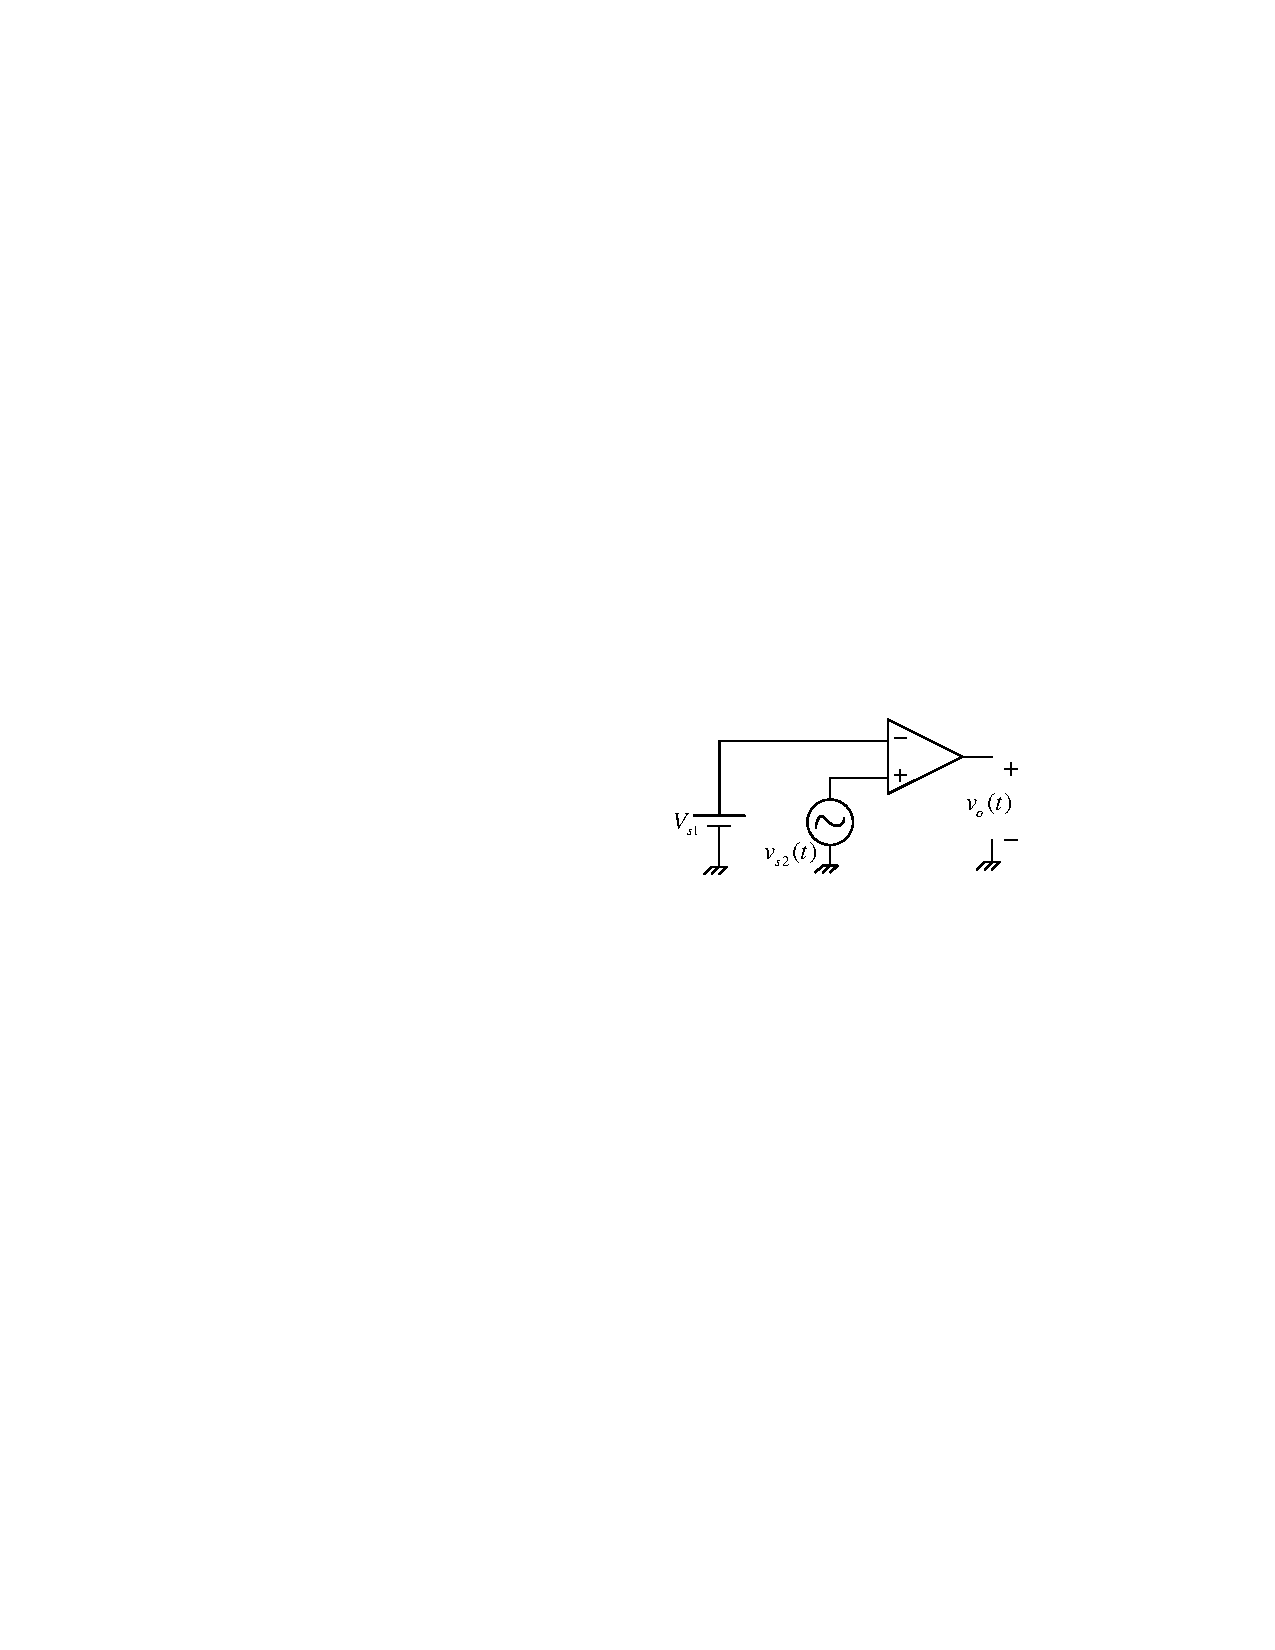
\includegraphics[scale=1.2,angle=0]{Fig/cir1.pdf}
        \caption{An op-amp as a comparator.} \label{fig:cir1}
    \end{figure}

    %--------------------------------------------
    \begin{subquestion}{Set $V_{s1}=0$ or equivalently, connect the inverting input of the op-amp to the ground. Apply a $1$-V $1$-kHz sine voltage $v_{s2}(t)$ to the non-inverting input. Watch the the output voltage and the non-inverting input voltage of the op-amp simultaneously on the oscilloscope. Interpret the results. Change the sine wave to a triangle wave and observe the results.}
        \answer{}
    \end{subquestion}

    %--------------------------------------------
    \begin{subquestion}{Set $V_{s1}=\pm 0.5$ V and repeat the previous part.}
        \answer{}
    \end{subquestion}

    %--------------------------------------------
    \begin{subquestion}{Swap the input voltages to the op-amp and redo the previous parts.}
        \answer{}
    \end{subquestion}


\end{question}

%----------------------------------------------------------------------------------------
%	QUESTION 2
%----------------------------------------------------------------------------------------

\begin{question}

    \questiontext{Build the circuit shown in Fig. \ref{fig:cir2} using an op-amp comparator module. Create a pair of $\pm 18$ V voltages and connect them to the supply connectors of the module as well as to the fixed legs of the potentiometer.}

    \begin{figure}[H]
        \centering
        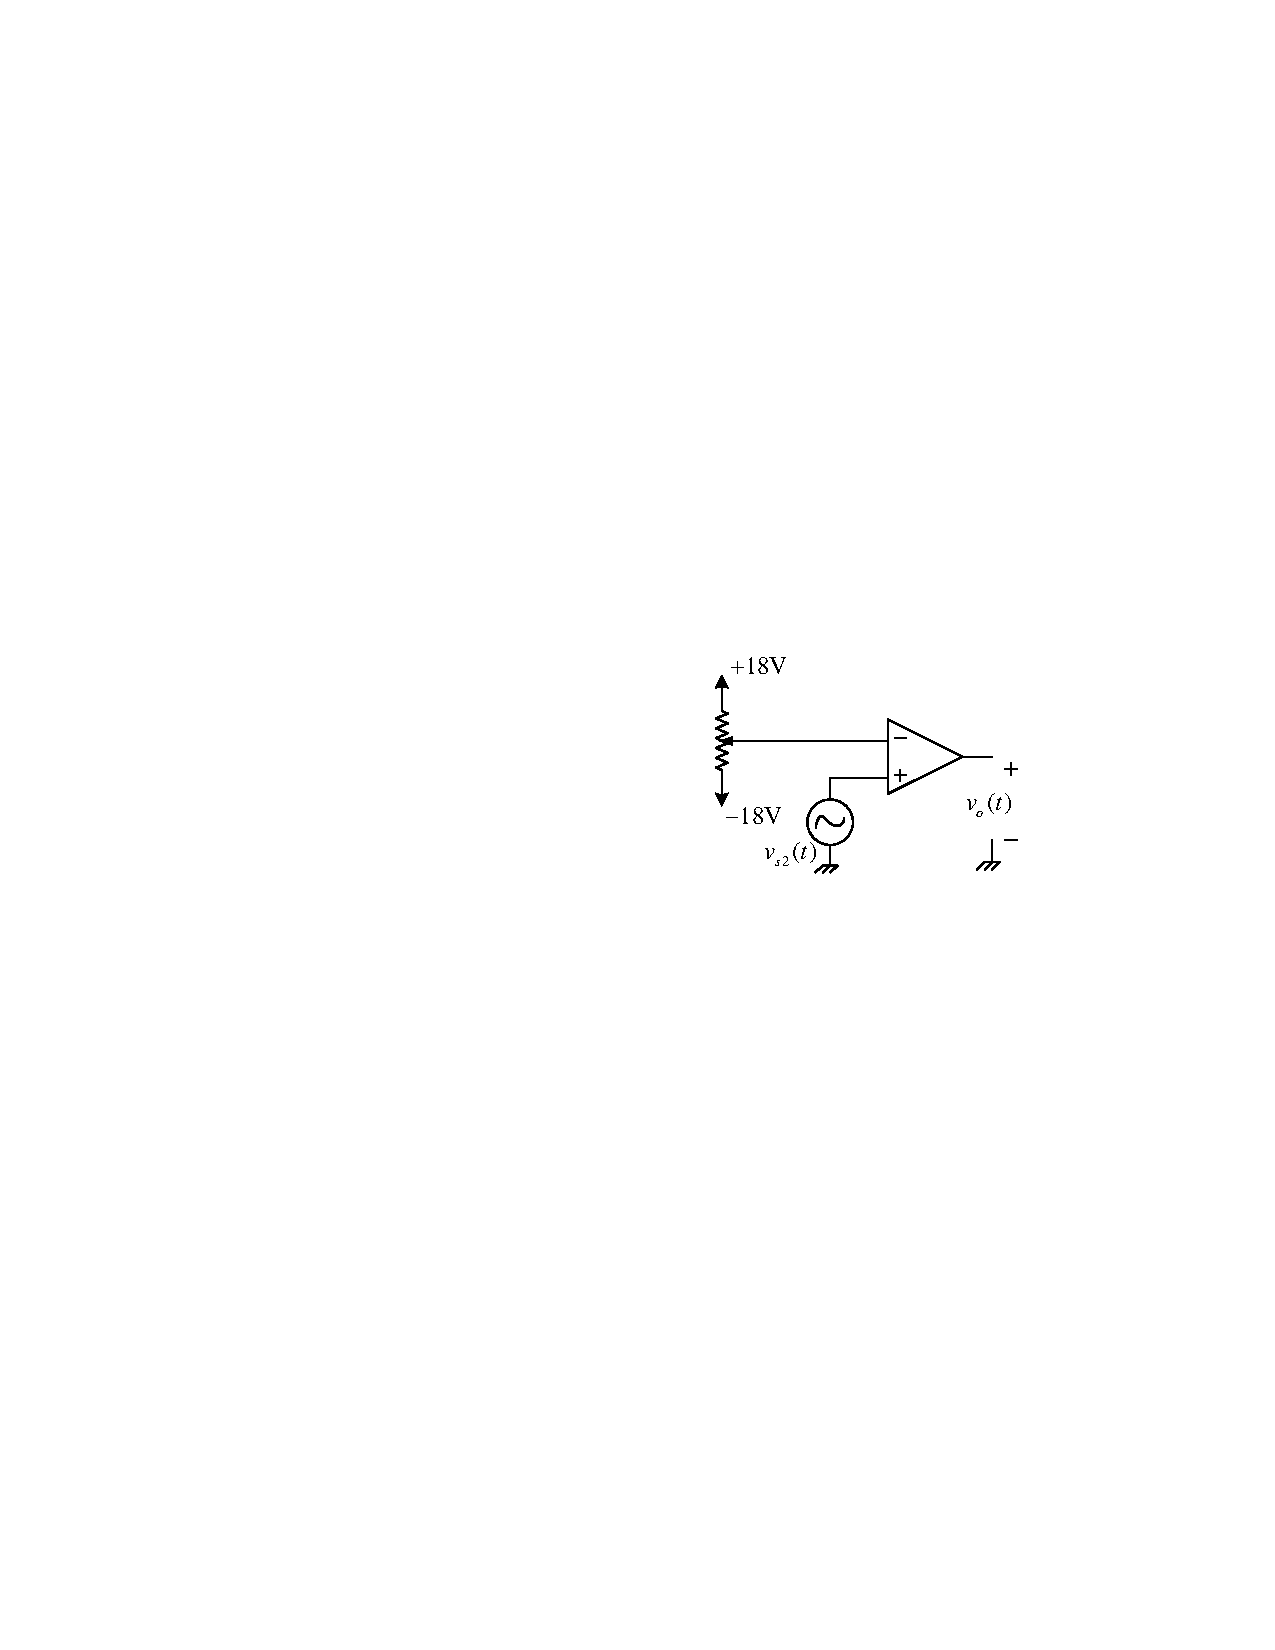
\includegraphics[scale=1.2,angle=0]{Fig/cir2.pdf}
        \caption{An op-amp as a comparator along with a potentiometer as a voltage divider.} \label{fig:cir2}
    \end{figure}

    %--------------------------------------------
    \begin{subquestion}{Apply a $1$-V $1$-kHz sine voltage $v_{s2}(t)$ to the non-inverting input. Watch the the output voltage and the non-inverting input voltage of the op-amp simultaneously on the oscilloscope. Turn the knob of the potentiometer and observe the results.}
        \answer{}
    \end{subquestion}

    %--------------------------------------------
    \begin{subquestion}{Repeat the previous part for a triangle wave.}
        \answer{}
    \end{subquestion}


\end{question}

%----------------------------------------------------------------------------------------
%	QUESTION 3
%----------------------------------------------------------------------------------------

\begin{question}

    \questiontext{Build the circuit shown in Fig. \ref{fig:cir3} using an op-amp inverting amplifier module. Create a pair of $\pm 18$ V voltages and connect them to the supply connectors of the module.}

    \begin{figure}[H]
        \centering
        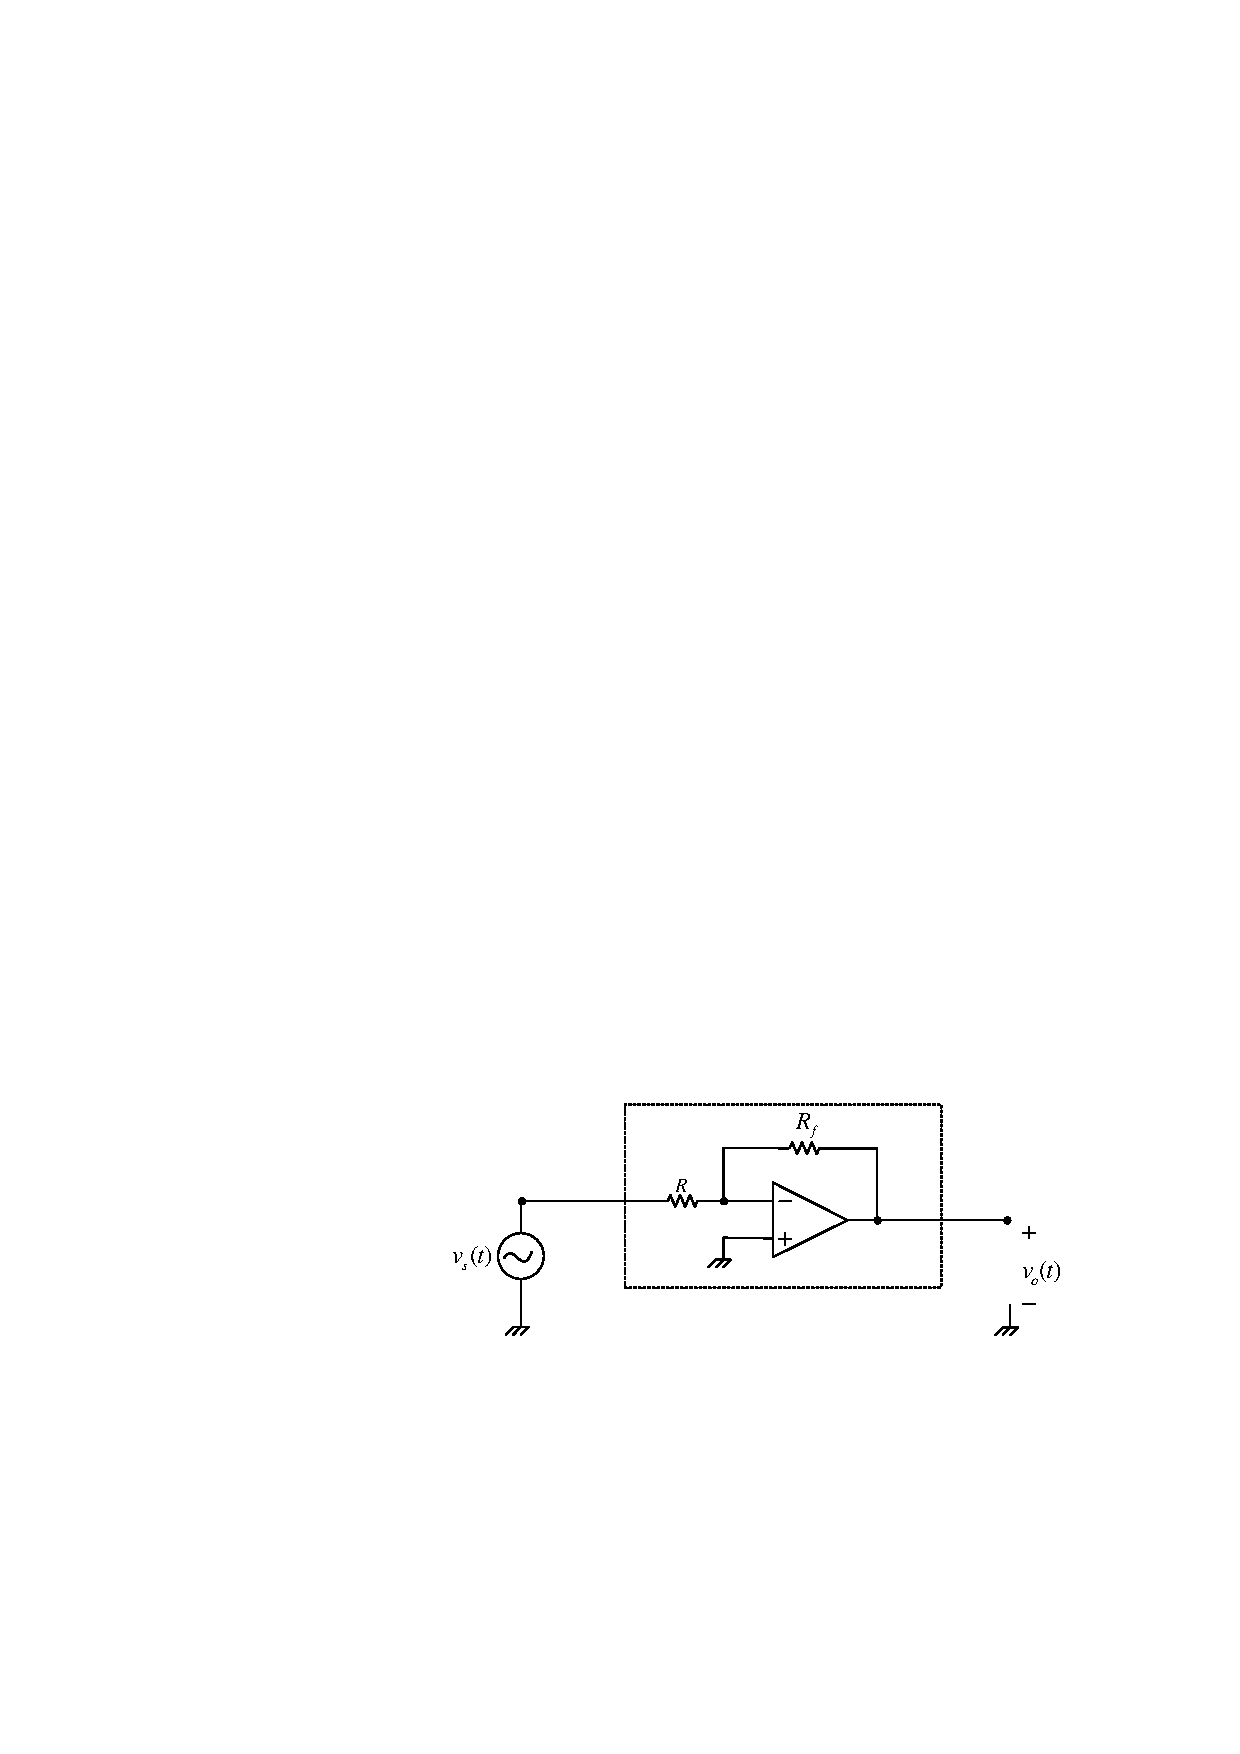
\includegraphics[scale=1.2,angle=0]{Fig/cir3.pdf}
        \caption{Inverting amplifier.} \label{fig:cir3}
    \end{figure}

    %--------------------------------------------
    \begin{subquestion}{Apply a $0.5$-V $1$-kHz sine voltage $v_{s}(t)$ to the input of the amplifier. Watch the the output and input voltages of the amplifier simultaneously on the oscilloscope. Calculate the gain of the amplifier.}
        \answer{}
    \end{subquestion}

    %--------------------------------------------
    \begin{subquestion}{Devise an experiment to measure the input and output resistance of the amplifier module.}
        \answer{}
    \end{subquestion}

    %--------------------------------------------
    \begin{subquestion}{Increase the amplitude of the input $1$-kHz sine wave and record your observations. Interpret and discuss the results.}
        \answer{}
    \end{subquestion}

    %--------------------------------------------
    \begin{subquestion}{Increase the frequency of the input $0.5$-V sine wave and record your observations. Interpret and discuss the results.}
        \answer{}
    \end{subquestion}

\end{question}


%----------------------------------------------------------------------------------------
%	QUESTION 4
%----------------------------------------------------------------------------------------

\begin{question}

    \questiontext{Build the circuit shown in Fig. \ref{fig:cir4} using an op-amp non-inverting amplifier module. Create a pair of $\pm 18$ V voltages and connect them to the supply connectors of the module.}

    \begin{figure}[H]
        \centering
        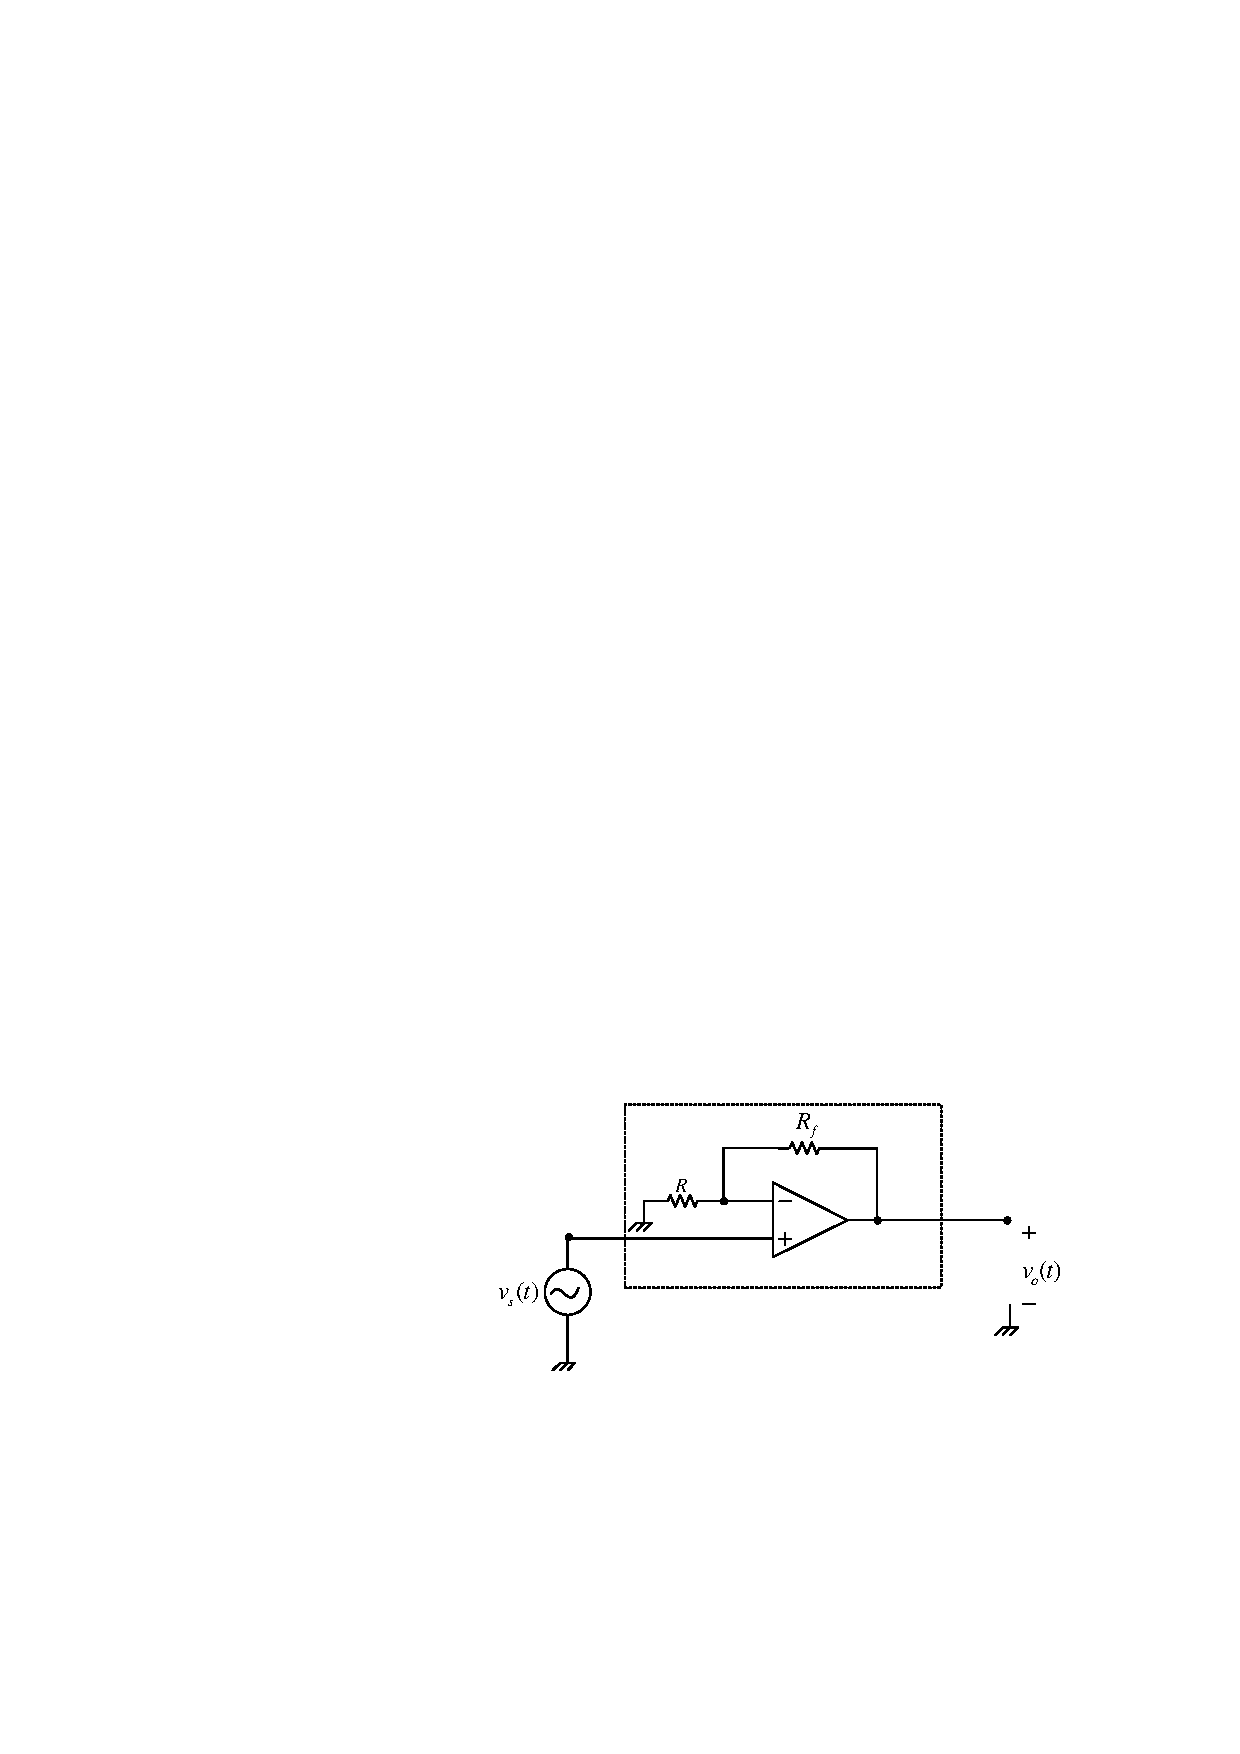
\includegraphics[scale=1.2,angle=0]{Fig/cir4.pdf}
        \caption{Non-inverting amplifier.} \label{fig:cir4}
    \end{figure}

    %--------------------------------------------
    \begin{subquestion}{Apply a $0.5$-V $1$-kHz sine voltage $v_{s}(t)$ to the input of the amplifier. Watch the the output and input voltages of the amplifier simultaneously on the oscilloscope. Calculate the gain of the amplifier.}
        \answer{}
    \end{subquestion}

    %--------------------------------------------
    \begin{subquestion}{Measure the input and output resistance of the amplifier module experimentally.}
        \answer{}
    \end{subquestion}

    %--------------------------------------------
    \begin{subquestion}{Increase the amplitude of the input $1$-kHz sine wave and record your observations. Interpret and discuss the results.}
        \answer{}
    \end{subquestion}

    %--------------------------------------------
    \begin{subquestion}{Increase the frequency of the input $0.5$-V sine wave and record your observations. Interpret and discuss the results.}
        \answer{}
    \end{subquestion}

\end{question}

%----------------------------------------------------------------------------------------
%	QUESTION 5
%----------------------------------------------------------------------------------------

\begin{question}

    \questiontext{Cascade an inverting amplifier and a non-inverting amplifier as shown in Fig. \ref{fig:cir5}}.

    \begin{figure}[H]
        \centering
        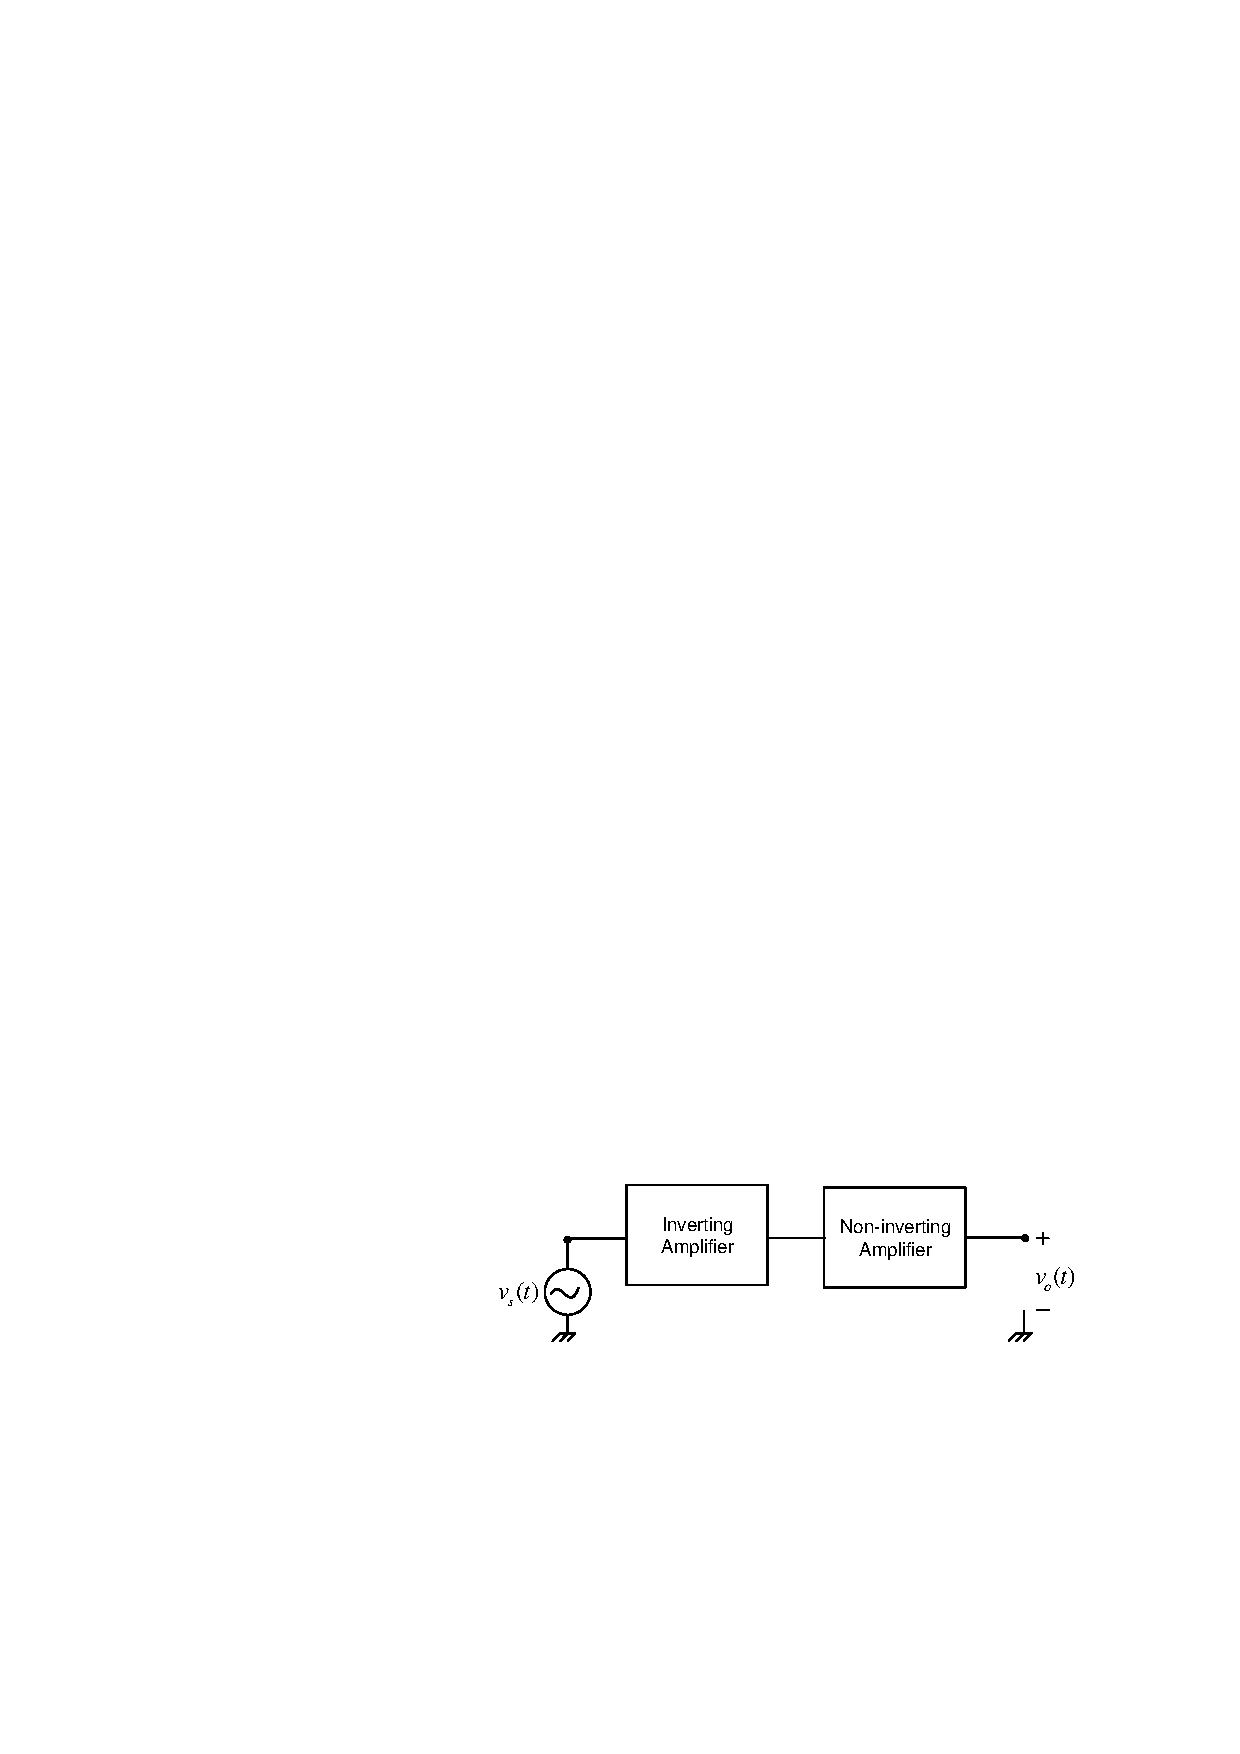
\includegraphics[scale=1.2,angle=0]{Fig/cir5.pdf}
        \caption{Cascade of two amplifiers.} \label{fig:cir5}
    \end{figure}

    %--------------------------------------------
    \begin{subquestion}{Apply a $100$-mV $1$-kHz sine voltage $v_{s}(t)$ to the input of the cascaded amplifiers. Watch the the output and input voltages of the cascaded amplifiers simultaneously on the oscilloscope. Calculate the overall gain of the cascaded amplifiers.}
        \answer{}
    \end{subquestion}

    %--------------------------------------------
    \begin{subquestion}{Swap the order of the amplifiers and repeat the previous part. Is there any difference between the measured gains in the two experiments? Explain.}
        \answer{}
    \end{subquestion}

\end{question}


\assignmentSection{Bonus Experiments}

%----------------------------------------------------------------------------------------
%	QUESTION 6
%----------------------------------------------------------------------------------------

\begin{question}

    \questiontext{In a circuit design, we need to cascade an inverting and a non-inverting amplifier to get the overall gain of $G_{tot}=G_{inv}G_{nnv}$. }

    %-------------------------------------------------------------
    \begin{subquestion}{From analytical point of view, is there any difference to change the order of the cascaded amplifiers?}
        \answer{}
    \end{subquestion}

    %-------------------------------------------------------------
    \begin{subquestion}{From practical point of view, is there any difference to change the order of the cascaded amplifiers? Justify your answer using PSpice simulation.}
        \answer{}
    \end{subquestion}

\end{question}


%----------------------------------------------------------------------------------------
%	QUESTION 7
%----------------------------------------------------------------------------------------
\begin{question}

    \questiontext{Op-amps usually need a pair of positive and negative DC supply voltages $\pm V_s$.}

    %-------------------------------------------------------------
    \begin{subquestion}{What happens if the absolute values of the supply voltages differ? }
        \answer{}
    \end{subquestion}

    %-------------------------------------------------------------
    \begin{subquestion}{Is it possible to use an op-amp with the supply voltages $0$ and $+V_s$? Explain.}
        \answer{}
    \end{subquestion}

\end{question}


%----------------------------------------------------------------------------------------
%	QUESTION 8
%----------------------------------------------------------------------------------------

\begin{question}

    \questiontext{Return your work report by filling the \LaTeX template of the manual. Include useful and high-quality images to make the report more readable and understandable.}

\end{question}

%----------------------------------------------------------------------------------------

\end{document}
